% Slides for a self-study report. Build with tools/build_slides.sh <study-dir>.
% Citations come from report/refs.bib via BIBINPUTS set by build_slides.sh.
% One message per frame; every number matches report/main.tex.
\documentclass[aspectratio=169,11pt]{beamer}

\usetheme{Madrid}
\usecolortheme{default}
\setbeamertemplate{navigation symbols}{}
\usepackage[T1]{fontenc}
\usepackage{amsmath,amssymb}
\usepackage{booktabs}
\usepackage{tikz}
\usetikzlibrary{positioning,arrows.meta}
\usepackage[numbers]{natbib}

\newcommand{\codex}[0]{Codex}
\newcommand{\occ}[0]{OpenCode}
\newcommand{\ccc}[0]{Claude Code}

% Beamer-safe inline code: no \path, keep tokens short.

\title[Coding-agent harnesses in three products]{How Claude Code, Codex, and OpenCode Build Their Coding-Agent Harnesses}
\subtitle{A static source-trace comparison at pinned commits}
\author[self-study-with-ai]{self-study-with-ai}
\date{\today}

\begin{document}

\begin{frame}
  \titlepage
  \note{One talk, one question: what is inside the harness that turns a
  language model into a coding agent, and how differently do the three
  products answer it?}
\end{frame}

\begin{frame}{Outline}
  \tableofcontents
\end{frame}

\section{Motivation}

\begin{frame}{Why study the harness?}
  \textbf{The interface layer is a first-order factor, not plumbing.}
  \begin{itemize}
    \item ReAct: interleaving reasoning and acting beats either alone;
      grounded search cut hallucinated failures from 56\% to 0\% on
      HotpotQA~\citep{yao2023react}.
    \item Toolformer: the interrupt, execute, resume protocol behind every
      tool call, with decoding constrained to stop tool-call
      loops~\citep{schick2023toolformer}.
    \item SWE-agent: an agent-tailored interface raised SWE-bench Lite
      resolution from 11.0\% (shell-only) to 18.0\% with GPT-4 Turbo;
      51.7\% of instances had a failed edit, and edit success dropped from
      90.5\% to 57.2\% after one failure~\citep{yang2024sweagent}.
  \end{itemize}
  \textbf{Gap.} We know interface design matters; we do not know how the
  shipping products practitioners use actually build it.
  \note{All three citations are the framing preprints; the SWE-agent
  numbers are the motivation for treating harness machinery as the object
  of study.}
\end{frame}

\begin{frame}{Research questions}
  \begin{enumerate}
    \item \textbf{RQ1 (primary).} How do \ccc{}, \codex{}, and \occ{}
      implement their coding-agent harnesses, and where do they genuinely
      differ?
    \item \textbf{RQ2.} What components make up a coding-agent harness?
    \item \textbf{RQ3.} How does each system trade capability against
      safety in shell and file access?
    \item \textbf{RQ4.} What does \ccc{}'s closed core reveal through
      documentation, its plugin surface, and third-party teardowns?
  \end{enumerate}
\end{frame}

\section{Study design}

\begin{frame}{Three systems, three evidence tiers}
  \begin{columns}[T]
    \column{0.32\textwidth}
      \textbf{\codex{}} (OpenAI, Apache-2.0)\\
      open source, pinned \texttt{af70018}\\
      evidence: \emph{pinned code}
    \column{0.32\textwidth}
      \textbf{\occ{}} (anomalyco, MIT)\\
      open source, pinned \texttt{d545d8f} (\texttt{dev})\\
      evidence: \emph{pinned code}
    \column{0.32\textwidth}
      \textbf{\ccc{}} (Anthropic)\\
      core closed; pinned surface \texttt{c3d2e35}\\
      evidence: \emph{docs snapshots + plugin surface}
  \end{columns}

  \medskip
  \textbf{Evidence discipline.}
  \begin{itemize}
    \item Static source traces only: nothing executed, no API called;
      checkouts treated as read-only untrusted data~\citep{codexRepo,opencodeRepo,claudeCodeSurface}.
    \item \ccc{} internals are boundaries, not findings; teardowns enter
      only as hedged context~\citep{minusXTeardown,agiflowInternals,tenguDecoded}.
  \end{itemize}
\end{frame}

\begin{frame}{Pre-registered trace experiments}
  Four frozen extractions (plan EXP-PLAN-2026-08-19-v1), every value
  carrying a file:line or snapshot-line anchor:
  \begin{center}
    \small
    \begin{tabular}{llr}
      \toprule
      Trace & Scope & Anchors re-verified\\
      \midrule
      E1 & turn loops & 59/59\\
      E2 & tool surfaces & 131/131\\
      E3 & safety policies & 75/75\\
      E4 & compaction parameters & 35/35\\
      \midrule
      & \textbf{total at the pinned commits} & \textbf{300/300}\\
      \bottomrule
    \end{tabular}
  \end{center}
  Validation runs are smoke-test plumbing; the extraction artifacts carry
  the findings. All three HEADs matched the pins at every validation.
\end{frame}

\section{Harness anatomy}

\begin{frame}{Eight machinery dimensions (RQ2)}
  \begin{columns}[T]
    \column{0.55\textwidth}
      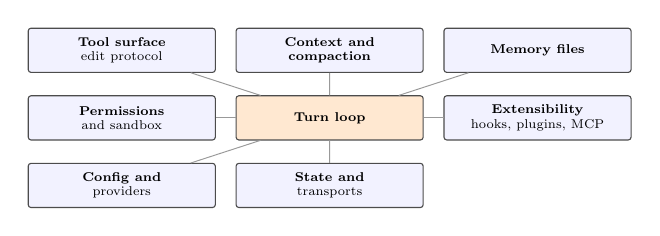
\begin{tikzpicture}[font=\scriptsize, scale=0.66, transform shape,
        box/.style={draw=black!70, rounded corners=1pt, align=center,
          minimum width=3.6cm, minimum height=0.85cm, inner sep=2pt,
          fill=blue!5, text=black},
        loop/.style={box, fill=orange!18},
        conn/.style={draw=black!40, line width=0.35pt}]
      \node[loop] (loop) at (0,0) {\textbf{Turn loop}};
      \node[box] (tools) at (-4.0, 1.3) {\textbf{Tool surface}\\edit protocol};
      \node[box] (ctx)   at ( 0.0, 1.3) {\textbf{Context and}\\\textbf{compaction}};
      \node[box] (mem)   at ( 4.0, 1.3) {\textbf{Memory files}};
      \node[box] (perm)  at (-4.0, 0) {\textbf{Permissions}\\and sandbox};
      \node[box] (ext)   at ( 4.0, 0) {\textbf{Extensibility}\\hooks, plugins, MCP};
      \node[box] (cfg)   at (-4.0,-1.3) {\textbf{Config and}\\providers};
      \node[box] (state) at ( 0.0,-1.3) {\textbf{State and}\\transports};
      \foreach \n in {tools,ctx,mem,perm,ext,cfg,state}
        \draw[conn] (loop) -- (\n);
      \end{tikzpicture}
    \column{0.42\textwidth}
      Every system implements all eight dimensions; they differ in
      \emph{how}:
      \begin{itemize}
        \item the abstraction is settled: loop, tools, compaction,
          permissions, extensions;
        \item the engineering culture is not: trust boundaries, state
          durability, interface unification.
      \end{itemize}
      Naming differences (hooks, skills, agents) overlay the structural
      ones rather than masking them.
  \end{columns}
  \note{This is RQ2. The decomposition is grounded in three pinned
  implementations and the framing literature; see the report's Table 1 for
  the full matrix.}
\end{frame}

\section{Findings}

\begin{frame}{Turn loops: one contract, three realizations (E1)}
  \small
  \begin{columns}[T]
    \column{0.32\textwidth}
      \textbf{\codex{}: abortable task state machine}
      \begin{itemize}
        \item \texttt{Op} enum, 27 variants; task kinds Regular, Review,
          Compact; preemption via \texttt{Replaced}~\citep{codexRepo}
        \item continue iff \texttt{needs\_follow\_up} = model bit OR
          pending input
        \item steering rejected via an 8-variant taxonomy
      \end{itemize}
    \column{0.32\textwidth}
      \textbf{\occ{}: persistence-driven loop}
      \begin{itemize}
        \item \texttt{while (true)} over persisted message parts; verdict
          compact / stop / continue~\citep{opencodeRepo}
        \item exit re-derived from stored state each iteration
        \item \texttt{doom\_loop} ask after 3 byte-identical calls;
          retry cap 5
      \end{itemize}
    \column{0.32\textwidth}
      \textbf{\ccc{}: closed core, docs-attested seams}
      \begin{itemize}
        \item hook cadences: per session, per turn, per tool
          call~\citep{claudeCodeHooksDocs}
        \item stop-hook override after 8 consecutive blocks
        \item continuation condition, caps, retries undisclosed
      \end{itemize}
  \end{columns}

  \medskip
  Same abstract loop and an explicit anti-loop defense in each system,
  realized three different ways.
\end{frame}

\begin{frame}{Tools and patches: the format converges (E2)}
  \begin{itemize}
    \item \textbf{Registration policy differs.} \codex{}: 32 conditional
      per-turn registrations behind feature and model gates. \occ{}:
      fixed array of 17 tool IDs. \ccc{}: 12 built-ins named in docs plus
      8 more attested by the pinned surface; full registry open~\citep{codexRepo,opencodeRepo,claudeCodeHooksDocs,claudeCodeSurface}.
    \item \textbf{The patch format converges across vendors.} \occ{}
      ports the \codex{} \texttt{apply\_patch} grammar verbatim (``Core
      types matching the Rust implementation'') and selects it for
      \texttt{gpt-*} model IDs, except \texttt{gpt-4} and
      \texttt{oss}~\citep{opencodeRepo}.
    \item \textbf{Edit robustness is engineered in.} \occ{}'s
      \texttt{edit} runs a 9-stage replacer cascade (similarity 0.65),
      an answer to the fragility SWE-agent measured~\citep{yang2024sweagent}.
    \item \textbf{Negative finding.} \codex{} has no dedicated
      read/glob/grep tools in the extracted registry; the shell carries
      inspection (bounded to the extraction scope).
  \end{itemize}
\end{frame}

\begin{frame}{Compaction: literal constants of different kinds (E4)}
  \small
  \begin{columns}[T]
    \column{0.48\textwidth}
      \textbf{\codex{}: fractional trigger}~\citep{codexRepo}
      \begin{itemize}
        \item auto-compact at 9/10 of the resolved window, on a 95\%
          effective window
        \item budgets: 20{,}000 user-message tokens locally; 64{,}000
          retained remotely
        \item rollover compacts mid-turn, then continues
      \end{itemize}
      \smallskip
      \textbf{\occ{}: reserved-buffer trigger}~\citep{opencodeRepo}
      \begin{itemize}
        \item fires at input limit minus min(20{,}000, max-output)
          tokens
        \item pruning-shaped: protects last 40{,}000 tokens of tool
          output; recent messages clamped to 25\% of usable (2{,}000 to
          15{,}000)
      \end{itemize}
    \column{0.48\textwidth}
      \textbf{\ccc{}: seams without numbers}
      \begin{itemize}
        \item \texttt{PreCompact}/\texttt{PostCompact} hooks with manual
          and auto triggers~\citep{claudeCodeHooksDocs}
        \item root CLAUDE.md is re-injected after \texttt{/compact};
          nested files are not~\citep{claudeCodeMemoryDocs}
        \item no numeric threshold anywhere in the pinned snapshots
      \end{itemize}
  \end{columns}
\end{frame}

\begin{frame}{Safety: three points on one axis (E3)}
  \footnotesize
  \begin{columns}[T]
    \column{0.32\textwidth}
      \textbf{\codex{}: prevent}
      \begin{itemize}
        \item OS sandbox (Seatbelt, bubblewrap, seccomp) plus Starlark
          rule engine, strictest-wins~\citep{codexRepo,codexSandboxingDocs}
        \item ships no usable policy file; trust-gated project config
      \end{itemize}
    \column{0.32\textwidth}
      \textbf{\occ{}: recover}
      \begin{itemize}
        \item in-process ruleset only; default \texttt{*}:~allow, narrow
          friction at dot-env reads and doom loops~\citep{opencodeRepo}
        \item no OS sandbox in the pinned tree; per-step snapshots with
          revert carry the safety story
      \end{itemize}
    \column{0.32\textwidth}
      \textbf{\ccc{}: layer}
      \begin{itemize}
        \item permission rules before every tool; OS sandbox scoped to
          Bash and its children only~\citep{claudeCodePermissionsDocs,claudeCodeSandboxingDocs}
        \item protected paths deny writes with no per-path exemption;
          enterprise kill switches
      \end{itemize}
  \end{columns}
\end{frame}

\begin{frame}{State and interfaces: convergence in shape, not substrate}
  \begin{itemize}
    \item \textbf{State.} \codex{}: append-only inspectable JSONL plus a
      repairable SQLite mirror; exact replay across compaction. \occ{}:
      event-sourced SQLite plus shadow-git file snapshots at every step.
      \ccc{}: undisclosed; only subagent transcripts documented (30-day
      cleanup default)~\citep{codexRepo,opencodeRepo,claudeCodeSubagentsDocs}.
    \item \textbf{Interfaces.} \codex{}: one JSON-RPC protocol behind
      every frontend. \occ{}: local HTTP server consumed by its TUI,
      plus ACP and 38 built-in LSP servers feeding diagnostics back into
      edits. \ccc{}: CLI, IDE, and desktop surfaces attested; transports
      closed~\citep{codexRepo,opencodeRepo,claudeCodePermissionsDocs}.
    \item \textbf{Extensibility converges on the \ccc{} design.}
      \codex{} exports \texttt{CLAUDE\_PLUGIN\_ROOT} compatibility and
      discovers \texttt{.claude-plugin} manifests; \occ{} reads
      \texttt{.claude} skill layouts~\citep{codexRepo,opencodeRepo}.
  \end{itemize}
\end{frame}

\section{Synthesis}

\begin{frame}{Converges vs. genuinely diverges}
  \begin{columns}[T]
    \column{0.48\textwidth}
      \textbf{Converges}
      \begin{itemize}
        \item the abstract prompt, sample, execute, continue loop
        \item structured edit protocols over free-form shell edits
        \item extension vocabulary: hooks, skills, agents, MCP
        \item dangerous defaults gated behind enterprise layers
      \end{itemize}
    \column{0.48\textwidth}
      \textbf{Genuinely diverges}
      \begin{itemize}
        \item control flow: state machine vs. persistence loop vs.
          closed loop
        \item tool registration: conditional vs. fixed vs. partly
          documented
        \item safety substrate: prevent vs. recover vs. layered
        \item compaction trigger: fraction vs. reserved buffer vs.
          undisclosed
        \item state: JSONL-first vs. SQL-event-first vs. undisclosed
      \end{itemize}
  \end{columns}
  \note{This is RQ1's answer: the naming layer converges while the
  substrate diverges on trust boundary placement, state durability, and
  interface unification.}
\end{frame}

\section{Limits and takeaways}

\begin{frame}{Limitations}
  \begin{itemize}
    \item \textbf{Version bounds.} Three pinned commits and docs
      snapshots of 2026-08-20; nothing generalizes to newer releases; the
      \occ{} pin is a \texttt{dev} branch.
    \item \textbf{No behavior measured.} Static by design: defaults and
      triggers describe code paths and contracts, not observed runtime.
    \item \textbf{Closed core.} \ccc{}'s loop, tool registry, compaction
      numbers, session storage, and enforcement internals remain open~\citep{claudeCodeSurface}.
    \item \textbf{Teardown tier.} Token counts and flag catalogs are
      unverified blog-tier assertions, used only as hedged context.
  \end{itemize}
\end{frame}

\begin{frame}{Takeaway}
  \begin{block}{Same abstraction, different engineering cultures}
    Three production harnesses implement the same eight-dimensional
    coding-agent harness. What distinguishes them is not the vocabulary
    but where each places its trust boundary, how durable it makes its
    state, and whether it unifies its interfaces behind one protocol.
  \end{block}
  \medskip
  Every claim above is bounded to the pinned commits
  (\texttt{af70018}, \texttt{d545d8f}, \texttt{c3d2e35}) and the
  documentation snapshots of 2026-08-20.
\end{frame}

\begin{frame}[allowframebreaks]{References}
  \footnotesize
  \bibliographystyle{plainnat}
  \bibliography{refs}
\end{frame}

\appendix

\begin{frame}{Backup: evidence ledger}
  \begin{itemize}
    \item 33 per-component notes; every claim anchored to file:line at
      pinned commits or snapshot lines.
    \item 12 claims advanced to ANALYZED with supported evidential
      status (\texttt{CLM-E1-1a} to \texttt{CLM-E4-3a});
      \texttt{CLM-E2-1b} corrected a registration count from 33 to 32
      during review.
    \item Pinned checkouts: \codex{} \texttt{af70018} (main), \occ{}
      \texttt{d545d8f} (dev), \ccc{} surface \texttt{c3d2e35} (main),
      pinned 2026-08-19.
  \end{itemize}
\end{frame}

\begin{frame}{Backup: open gaps (evidence, not absence)}
  \begin{itemize}
    \item \ccc{}: numeric compaction thresholds; turn-loop
      implementation; full tool registry; provider plumbing; sandbox
      enforcement internals.
    \item \occ{}: permission merge precedence; runtime enforcement of
      several schema defaults.
    \item \codex{}: remote model-catalog and enterprise cloud-bundle
      contents (server-side state).
    \item Exception: absence of an OS sandbox in the pinned \occ{} tree
      is a searched-scope result, not a gap.
  \end{itemize}
\end{frame}

\begin{frame}{Backup: teardown claims held at context tier}
  \begin{itemize}
    \item Intercepted-log teardown: system-prompt and tool-token sizes,
      small-model routing (unverified)~\citep{minusXTeardown}.
    \item Binary analysis: 243 feature flags, 1{,}163 telemetry events,
      49 built-in tools at one version (unverified)~\citep{tenguDecoded}.
    \item Trace-based breakdown: CLAUDE.md delivery shape, cross-verified
      against official memory docs; only that overlap is reinforced~\citep{agiflowInternals,claudeCodeMemoryDocs}.
  \end{itemize}
\end{frame}

\end{document}
